\documentclass[DM,lsstdraft,authoryear,toc]{lsstdoc}
% lsstdoc documentation: https://lsst-texmf.lsst.io/lsstdoc.html

% Package imports go here.
\usepackage{booktabs}
\usepackage{xspace}
\usepackage{hyperref}
\usepackage{graphicx}
\usepackage{makecell}

% Local commands go here.
\newcommand{\opsim}{\texttt{OpSim}\xspace}
\newcommand{\socs}{\texttt{SOCS}\xspace}
\newcommand{\sched}{\texttt{Scheduler}\xspace}
\newcommand{\simsky}{\texttt{sims\_skybrightness}\xspace}
\newcommand{\magasq}{magnitude/arcsecond$^{2}$\xspace}

% To add a short-form title:
% \title[Short title]{Title}
\title{Alternate observing strategies}

% Optional subtitle
% \setDocSubtitle{A subtitle}

\author{%
Owen Boberg,
Lynne Jones,
Tiago Ribeiro, \\
\v{Z}eljko Ivezi\'{c}}

\setDocRef{alternate-strategies}

\date{\today}

% Optional: name of the document's curator
% \setDocCurator{The Curator of this Document}

%\setDocAbstract{%
%We now describe some alternatives to the Baseline Cadence that were explored. These OpSim databases are all available for further testing with science-based MAF metrics.}

% Change history defined here.
% Order: oldest first.
% Fields: VERSION, DATE, DESCRIPTION, OWNER NAME.
% See LPM-51 for version number policy.
\setDocChangeRecord{%
  \addtohist{1}{YYY-MM-DD}{Unreleased.}{Owen Boberg}
}

\begin{document}

% Create the title page.
% Table of contents is added automatically with the "toc" class option.
\maketitle

\section{Introdcution}

Here we will present a series of new simulations that were used to test different survey strategies and rolling cadences.
All of the runs will be compared to kraken\_2026, which will soon be the official replacement for baseline2018a. There is
a separate document describing what changes were made to kraken\_2026 relative to baseline2018a, and how these changes
improve the survey performance. The purpose of this document is give an overall impression of how each new survey strategy 
compared to kraken\_2026 rather than go into the fine details. A list of the surveys is given in Table \ref{tab:runlist} along with
a short summary of how the survey was configured. In this document we will use the following when referring to the various
proposal in the surveys: Wide Fast Deep (WFD), Galactic Plane (GP), South Celestial Pole (SCP), North Ecliptic Spur (NES),
Deep Drilling Fields (DDFs).

\begin{table}[htp]
\caption{List simulated alternate observing strategies}
\begin{center}
\footnotesize
\begin{tabular}{| l | l | c |}
\toprule
\opsim Run & Summary  & Section \\
\midrule
kraken\_2026      & New Baseline Cadence using dome crawl and 36 second CL dealy & \\
\midrule
colossus\_2665   & Minimum and Maximum declination limits of WFD increased by $1.5^{\circ}$ & \ref{colossus2665} \\
\midrule
pontus\_2002      & PanSTARRs like survey, WFD and DD only, (X<1.5, DecMin = $-78^{\circ}$, DecMax = $+18^{\circ}$) & \ref{pontus2002}  \\  
\midrule
colossus\_2664   & WFD cadence through Galactic plane (GP), GP proposal removed from simulation & \ref{colossus2664} \\
\midrule
colossus\_2667   & No pairs survey &  \ref{colossus2667} \\
\midrule
pontus\_2489      & \makecell{"Many Visits" survey. 20s visits with single snap in g,r,i,z,y, \\ 40s visits with single snap in u}  &  \ref{pontus2489} \\
\midrule
kraken\_2035      &\makecell{ 9 Deep Drilling Fields (DDFs), \\ 4 already set DDFs + 5 new fields} &  \ref{kraken2035} \\
\midrule
mothra\_2045      & \makecell{Rolling cadence: 2 dec bands alternating every year. \\ Regular WFD removed} & \ref {mothra2045} \\
\midrule
pontus\_2502      &  \makecell{Rolling cadence: 2 dec bands alternating every year.  \\ Regular WFD at 25$\%$ level} & \ref {pontus2502} \\
\midrule
kraken\_2036      & \makecell{ Rolling cadence: Full WFD during first 2, and last two years, \\ 3 dec bands alternating every year in between} & \ref {kraken2036} \\
\bottomrule
\end{tabular}
\end{center}
\label{tab:runlist}
\end{table}

\section{Some Simulated Alternative Observing Strategies}

We now describe some alternatives to kraken\_2026 that were explored. 
These \opsim databases are all available for further testing with science-based MAF metrics.

\subsection{colossus\_2665} \label{colossus2665}

\textbf{Minimum and Maximum declination limits of WFD increased by $1.5^{\circ}$}

\textbf{Motivation and description}: The visits in \opsim v4 runs are pinned to a fixed tessellation on the sky without any transitional dithering pattern.
Using MAF, we are able to apply dithering patterns after the fact in order to smooth out the visit coverage over the sky. This can cause an issue because
visits can be pushed out of the main survey footprint, which in turn causes the fO metrics to fall below the SRD requirements. In colossus\_2665
we increased the maximum declination limit of the WFD survey to $4.3^{\circ}$ and decreased the minimum declination limit to $-64^{\circ}$. The dec
limits of the SCP and NES proposal were also adjusted to match the new limits of the WFD area. The motivation for slightly increasing the WFD
area was to produce a new baseline simulation that would pass the fO SRD requirements, even when the fields are dithered. .


\textbf{Expectations:} By expanding the WFD declination limits we expect that we can reduce the number of visits that are removed from 
the main survey footprint after dithering, and therefore still pass the fO SRD requirements. We also expect that this small change will not have a large 
effect on the overall performance of colossus\_2665 relative to kraken\_2026.

\textbf{Analysis and Results: Comparison of colossus\_2665 to kraken\_2026:} In Table~\ref{tab:srd-comparison-2665} we list the
fO metrics without (top portion) and with (bottom portion) dithering applied by MAF. As a reminder, the fO metric evaluates the overall 
efficiency of observing. \textbf{foNv}: out of 18000.00 sq degrees, the area receives at least X and  a median of Y visits (out of 825, 
if compared to benchmark). \textbf{fOArea}: this many sq deg (out of 18000.00 sq deg if compared to benchmark) receives at least 825 visits.
In Figure \autoref{fig:dither_nvisits-2665} we plot the total number of visits in all bands using the RandomDitherPerNight schema from MAF.

\begin{table}[htp]
\caption{Comparison of SRD metrics between kraken\_2026 and baseline2018a.}
\begin{center}
\small
\begin{tabular}{lrr}
\toprule
{}                                                                                       &   kraken\_2026 & colossus\_2665   \\
\midrule
 fOArea fO WFD                                           &      18040.6	&17783.8  \\
 fOArea/benchmark fO WFD                        &         1.002	& 0.988   \\
 fONv MedianNvis fO WFD                          &          938	& 907     \\
 fONv MinNvis fO WFD                                &            857	& 824     \\
 fONv/benchmark MedianNvis fO WFD       &         1.137	& 1.099  \\
 fONv/benchmark MinNvis fO WFD             &         1.039	& 0.999    \\
 \midrule
 With dithering random dithering per night    &  & \\
 fOArea fO WFD                                           &      17422.9	& 18827.9  \\
 fOArea/benchmark fO WFD                        &         0.968	& 1.046   \\
 fONv MedianNvis fO WFD                          &          1123	& 1078    \\
 fONv MinNvis fO WFD                                &           504	& 1009     \\
 fONv/benchmark MedianNvis fO WFD       &          1.361	& 1.307 \\
 fONv/benchmark MinNvis fO WFD             &         0.611	& 1.223   \\

\bottomrule
\end{tabular}
\end{center}
\label{tab:srd-comparison-2665}
\end{table}

\begin{enumerate}
\item The total number of visits in colossus\_2665 is 2.43 million relative to the 2.44 million in kraken\_2026.
\item The median total number of visits per HealPix in the WFD is slightly reduced in colossus\_2665 relative to kraken\_2026 (903 vs 938).
\item The median number of visits per night are 803 and 806 for colossus\_2665 and kraken\_2026, respectively.
Both simulations have a median slew time of 4.79 seconds.
\item The median seeing, sky brightness and airmass in the r and i bands are essentially the same between the two runs.
\item The median trigonometric parallax and proper motion errors are essentially the same.
\item There was not a significant change in the faction of total visits used by other proposals (e.g. NES, GP, DDFs, SCP).
\end{enumerate}

\begin{figure}[ht]
\centering
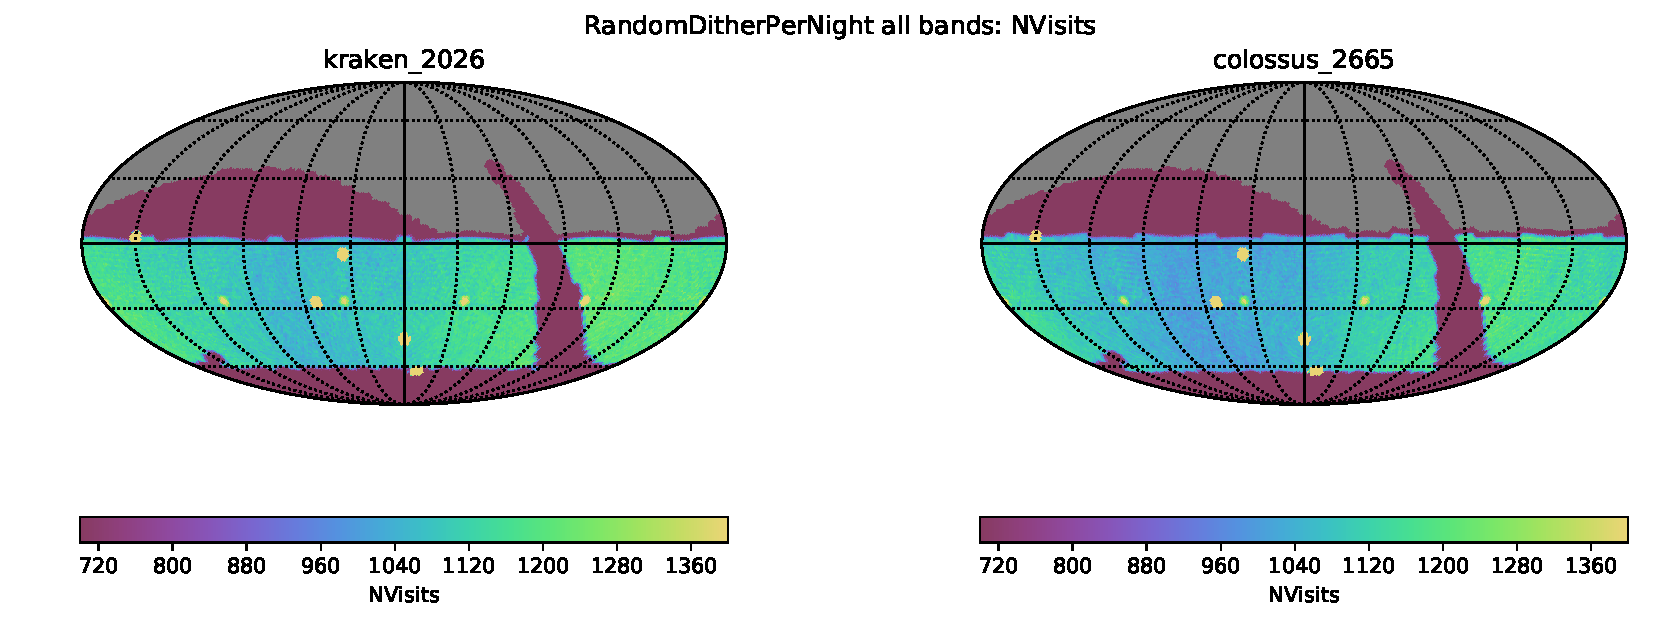
\includegraphics[width=0.98\textwidth]{figures/colossus_2665_kraken_2026_NVisits_RandomDitherPerNight_all_bands_HEAL_ComboSkyMap.pdf}
%\vskip -1.3in
\caption{Nvisits in all bands for kraken\_2026 (left) and colossus\_2665 (right).}
\label{fig:dither_nvisits-2665}
\end{figure}

\textbf{Conclusions:} By slightly extending the WFD footprint we can generate a simulation that passes the fO SRD
requirement when dithering is applied using MAF. This is an improvement over kraken\_2026 which fails the fONv MinNvis metric 
when dithering is applied. The slightly increased WFD footprint did cause any other major changes to the overall cadence and
performance of the survey. colossus\_2665 could be considered as a replacement for kraken\_2026 in the future.

\subsection{pontus\_2002} \label{pontus2002}

\textbf{Pan-STARRS-like survey + DDFs} 

\textbf{Motivation and description:}``Pan-STARRS-like cadence'' attempts to apply a uniform cadence strategy 
throughout the survey region, which is maximized and defined by DecMin = $-78^{\circ}$, DecMax = $+18^{\circ}$ deg (about 27,400 deg2). 
This is similar to the Pan-STARRS 3PI survey which tries to maximize sky area. The maximum acceptable airmass 
is kept at its default value of 1.5. This simulation utilizes WFD and DDFs, but no other proposals. 
This survey, like kraken\_2026, still required pairs of visits.

\textbf{Expectations:} The total number of visits in pontus\_2002 should be approximately the same as kraken\_2026,
but covering a main survey area over a $42\%$ more sky. Given the larger area, we also expect there to be
fewer visits per field.

\textbf{Analysis and Results: Comparison of pontus\_2002 to kraken\_2026:}

\begin{enumerate}
\item The total number of visits in pontus\_2002 is 2.43 million relative to the 2.44 million in kraken\_2026. See \autoref{fig:nvisits-2002}
for a comparison of the number of visit maps for each survey. This figure also give a sense of the how the survey footprint is changed
in pontus\_2002.
\item The median total number of visits per HealPix in the WFD is reduced in pontus\_2002 relative to kraken\_2026 (696 vs 938).
\item The median number of visits per night is 804 and 806 for colossus\_2665 and kraken\_2026, respectively.
Both simulations have essentially the same slew time.
\item The median trigonometric parallax and proper motion errors show uniform behavior over the entire enlarged area 
(see Figure \autoref{fig:parallax-pm-2002}), with the values similar to those obtained for kraken\_2026.
\item The fraction of total visits in the WFD is 0.96 in pontus\_2002 and 0.86 in kraken\_2026. The fraction of visits
in the DDFs remained approximately the same at 0.04.
\item The median coadded depths in pontus\_2002 are 0.20, 0.19, 0.18, 0.16, 0.15, 0.16 (u,g,r,i,z,y) magnitudes fainter relative 
to kraken\_2026 in the WFD area.
\item The median airmass in all bands increases by 0.04 in pontus\_2002 relative to kraken\_2026 in the WFD area.
\end{enumerate}


\begin{figure}[ht]
\centering
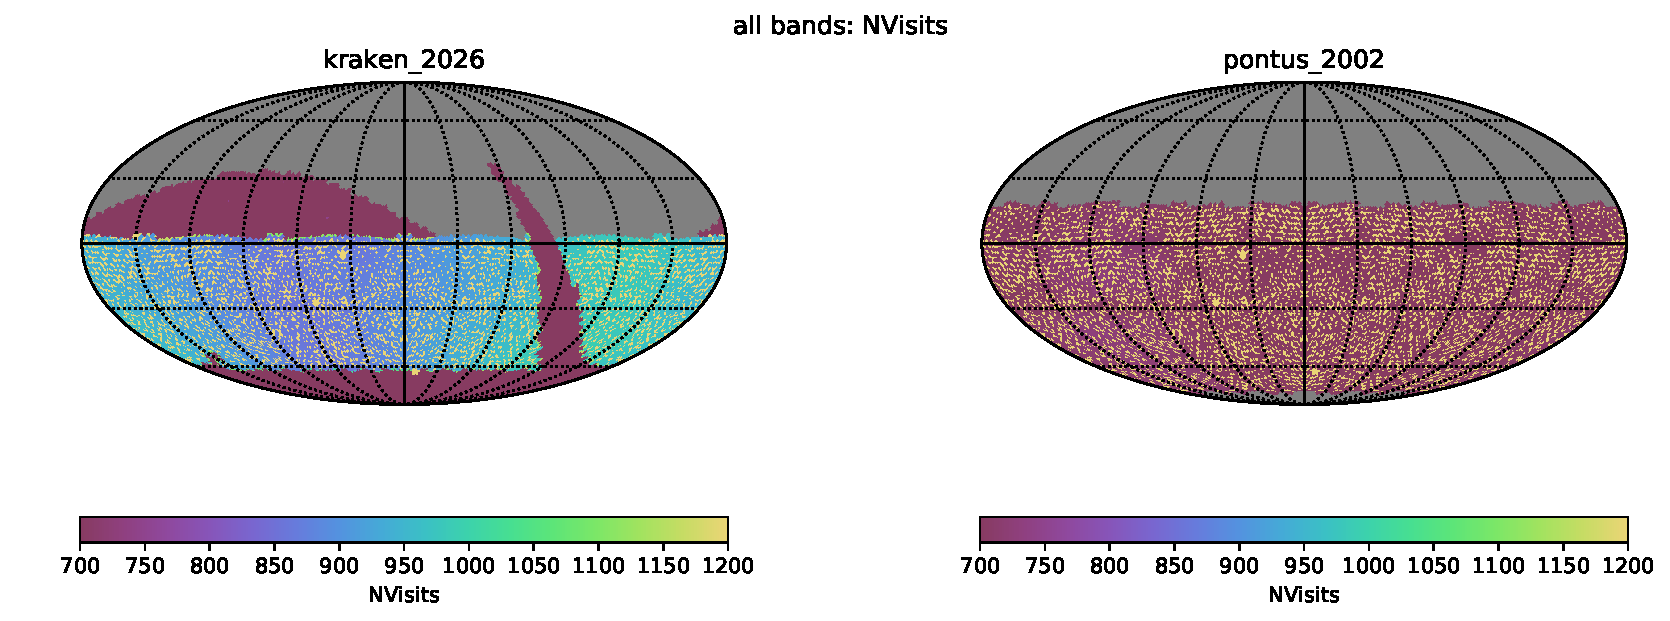
\includegraphics[width=0.98\textwidth]{figures/pontus_2002_kraken_2026_NVisits_all_bands_HEAL_ComboSkyMap.pdf}\\
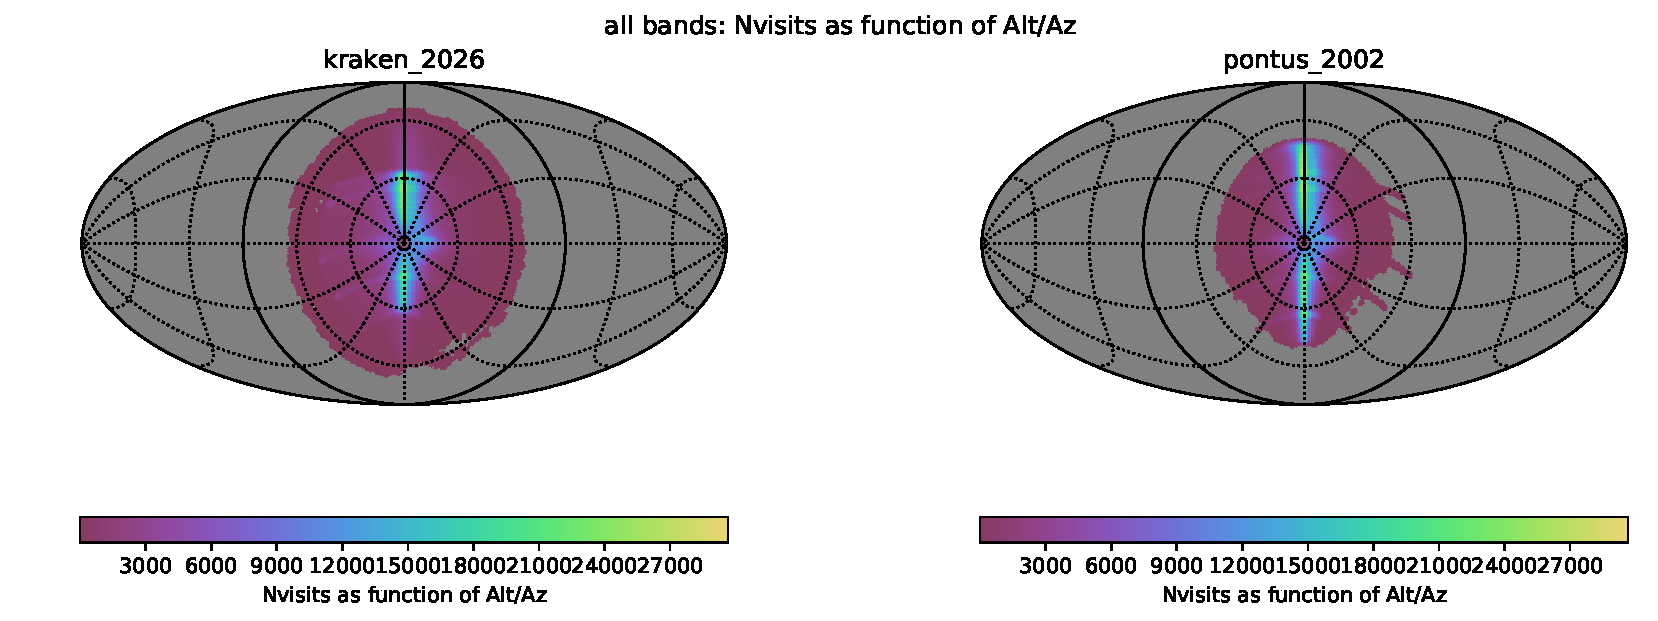
\includegraphics[width=0.98\textwidth]{figures/pontus_2002_kraken_2026_Nvisits_as_function_of_Alt_Az_all_bands_HEAL_ComboSkyMap.pdf}
%\vskip -1.3in
\caption{Skymaps for the number of visits in all bands. The maps for kraken\_2026 are in the left column and the maps for pontus\_2002 are
in the left column.}
\label{fig:nvisits-2002}
\end{figure}

\begin{figure}[ht]
\centering
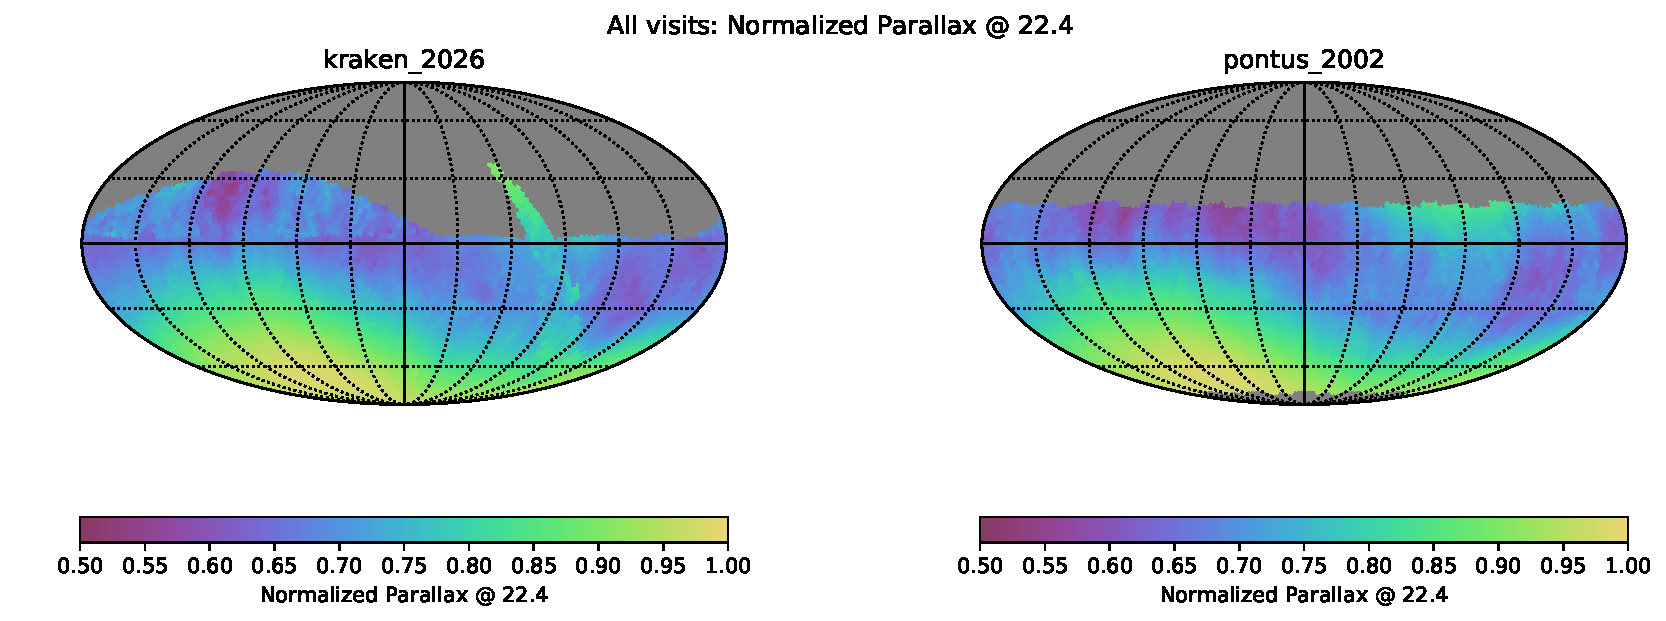
\includegraphics[width=0.98\textwidth]{figures/pontus_2002_kraken_2026_Normalized_Parallax_22_4_All_visits_HEAL_ComboSkyMap.pdf}\\
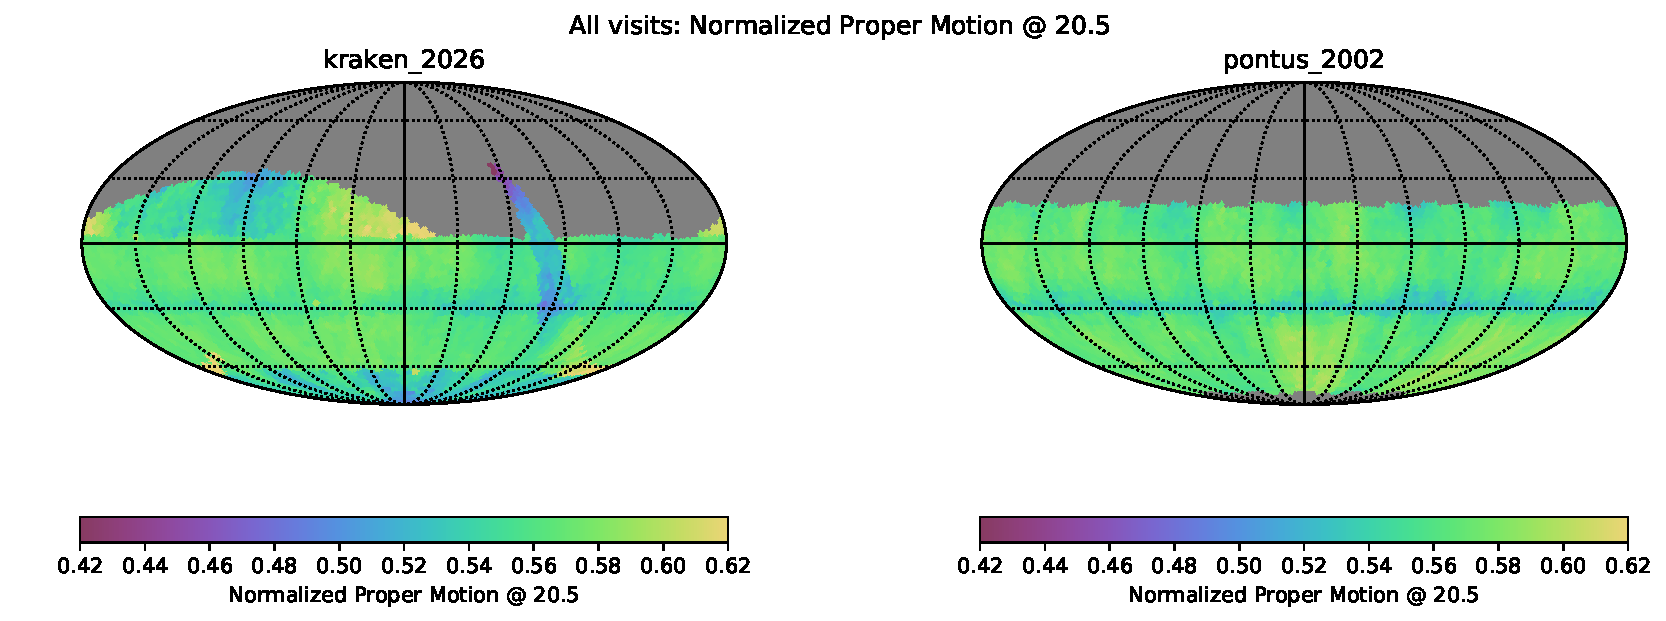
\includegraphics[width=0.98\textwidth]{figures/pontus_2002_kraken_2026_Normalized_Proper_Motion_20_5_All_visits_HEAL_ComboSkyMap.pdf}
%\vskip -1.3in
\caption{Top: Normalized parallax values at 22.4 mags for kraken\_2026 and pontus\_2002. Bottom: Normalized proper motion values
at 20.5 magnitudes for kraken\_2026 and pontus\_2002.}
\label{fig:parallax-pm-2002}
\end{figure}

\textbf{Conclusions:} pontus\_2002 increases survey area of the WFD by approximately 40$\%$ at the cost of fainter coadded depths in 
all bands. The loss of depth reduces the galaxy counts at a fixed SNR, but the increase survey area makes up for the loss in depth. The
larger median airmass and seeing also reduces the galaxy counts.

\subsection{colossus\_2664} \label{colossus2664}

\textbf{WFD cadence through GP, GP proposal removed from simulation}

\textbf{Motivation and description:} The goal of this simulation was to understand the effect of extending the
WFD cadence through the GP. This was configured by removing the GP avoidance region from the WFD
and SCP, and removing the GP from the list of available proposals.

\textbf{Analysis and Results: Comparison of colossus\_2664 to kraken\_2026:}

\begin{enumerate}
\item The total number of visits in the two simulations is essentially the same. See \autoref{fig:nvisits-2664}
for a comparison of the Nvisit maps for each survey.
\item The median total number of visits per HealPix in the WFD is reduced in colossus\_2664  relative to kraken\_2026 (887 vs 938).
\item The total number of visits in the WFD area increases by approximately 2$\%$ in colossus\_2664 relative to kraken\_2026
\item The median coadded depths in colossus\_2664 are 0.03, 0.03, 0.02, 0.02, 0.01, 0.03 (u,g,r,i,z,y) magnitudes shallower relative 
to kraken\_2026 in the WFD area.
\end{enumerate}

\begin{figure}[ht]
\centering
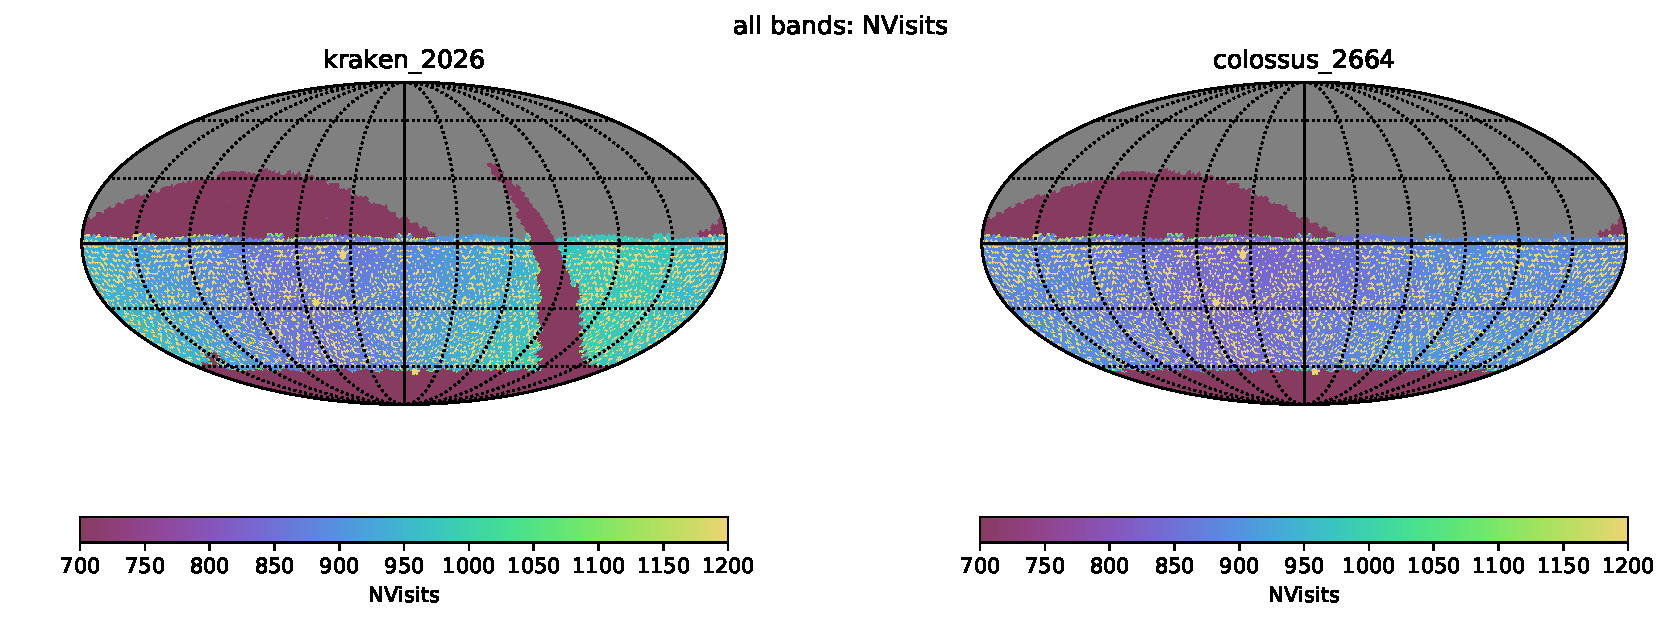
\includegraphics[width=0.98\textwidth]{figures/kraken_2026_colossus_2664_NVisits_all_bands_HEAL_ComboSkyMap.pdf}\\
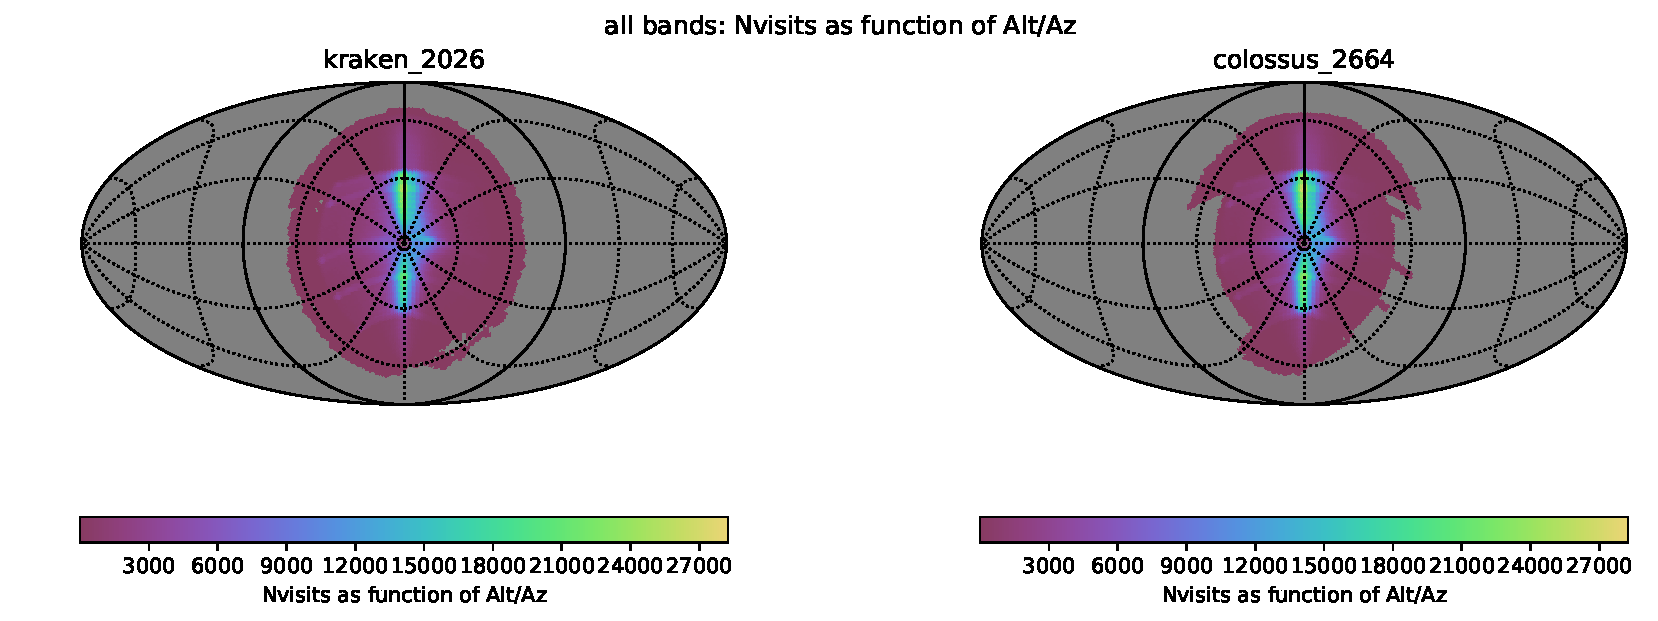
\includegraphics[width=0.98\textwidth]{figures/kraken_2026_colossus_2664_Nvisits_as_function_of_Alt_Az_all_bands_HEAL_ComboSkyMap.pdf}
%\vskip -1.3in
\caption{Skymaps for the number of visits in all bands. The maps for kraken\_2026 are in the left column and the maps for colossus\_2664 are
in the left column.}
\label{fig:nvisits-2664}
\end{figure}

\textbf{Conclusions:} By extending the WFD cadence through the GP, the WFD makes up approximately 88$\%$ of the total number of visits.
The increased area of the WFD reduced the median number of visits in the WFD by approximately 5$\%$, which decreases the coadded depth
by about 0.03 magnitudes.

\subsection{colossus\_2667} \label{colossus2667}

\textbf{No pairs survey}

\textbf{Motivation and description:} The goal of this simulations was to determine how requiring visits in a pairs
impacts the overall survey efficiency. The only difference between the configuration of colossus\_2667
and kraken\_2026 is the removal of the visits in pairs requirement.

\textbf{Analysis and Results: Comparison of colossus\_2667 to kraken\_2026:}

\begin{enumerate}
\item The total number of visits in colossus\_2667 is 2.5 million, which is a $2.2\%$ increase relative to kraken\_2026.
\item The mean slew time is 5.8 sec in colossus\_2667 compared to 6.8 sec in kraken\_2026.
See \autoref{fig:slew-2667} for a comparison of their slew time histograms.
\item The total open shutter fraction increased in colossus\_2667 (0.75 vs 0.73).
\end{enumerate}

\begin{figure}[ht]
\centering
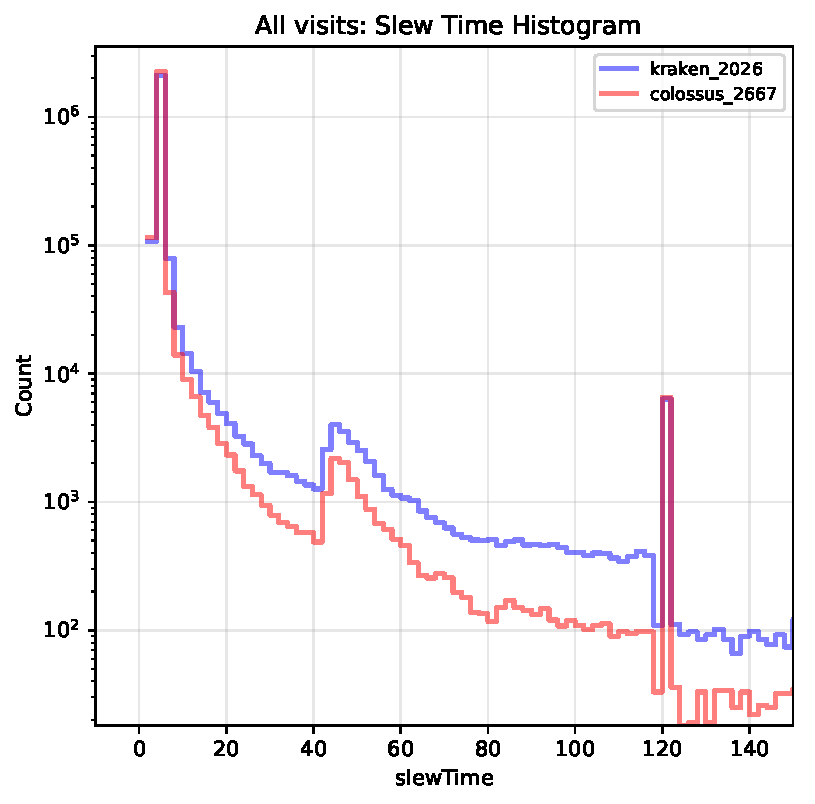
\includegraphics[width=0.65\textwidth]{figures/kraken_2026_colossus_2667_Slew_Time_Histogram_All_visits_ONED_ComboBinnedData.pdf}
%\vskip -1.3in
\caption{Slew time histograms for colossus\_2667 and kraken\_2026 .}
\label{fig:slew-2667}
\end{figure}

\textbf{Conclusions:} Removing the pair requirement reduced the mean slew time by 1 second and increased the number of
visits by $2.2\%$.

\subsection{pontus\_2489} \label{pontus2489}

\textbf{Many visits survey}

\textbf{Motivation and description:} This survey was designed to use single 20 second snaps in
g,r,i,z,y, and single 40 second snaps in u. In kraken\_2026, and the rest of the simulations present in this document, 
a visit is composed of 2 back-to-back 15 second exposures giving the nominal 30 second exposure per visit. 

\textbf{Analysis and Results: Comparison of pontus\_2489 to kraken\_2026:}

\begin{enumerate}
\item The total number of visits in pontus\_2489 is 3.41 million, which is a $40\%$ increase relative to kraken\_2026.
\item The total open shutter fraction of both simulations is essentially the same.
\item The median fraction of visits in pairs in gri increased to 0.90 in pontus\_2489 from 0.87 in kraken\_2026.
\item The median number of visits in all bands in the WFD increased by $41\%$ relative to kraken\_2026.
\item The median u band coadded depth reached 0.44 mags deeper in kraken\_2026 (26.09 vs. 25.65). 
\item  The median g,r,i,y, and z coadded depths are 0.13, 0.08, 0,05, 0.08, 0.07 mags, respectively, shallower than kraken\_2026.
See Figure  \autoref{fig:ubandhist-2489} and Figure  \autoref{fig:ubandmap-2489} for comparisons of the coadded u band
HealPix histograms and sky maps, resepctively.
\end{enumerate}

\begin{figure}[ht]
\centering
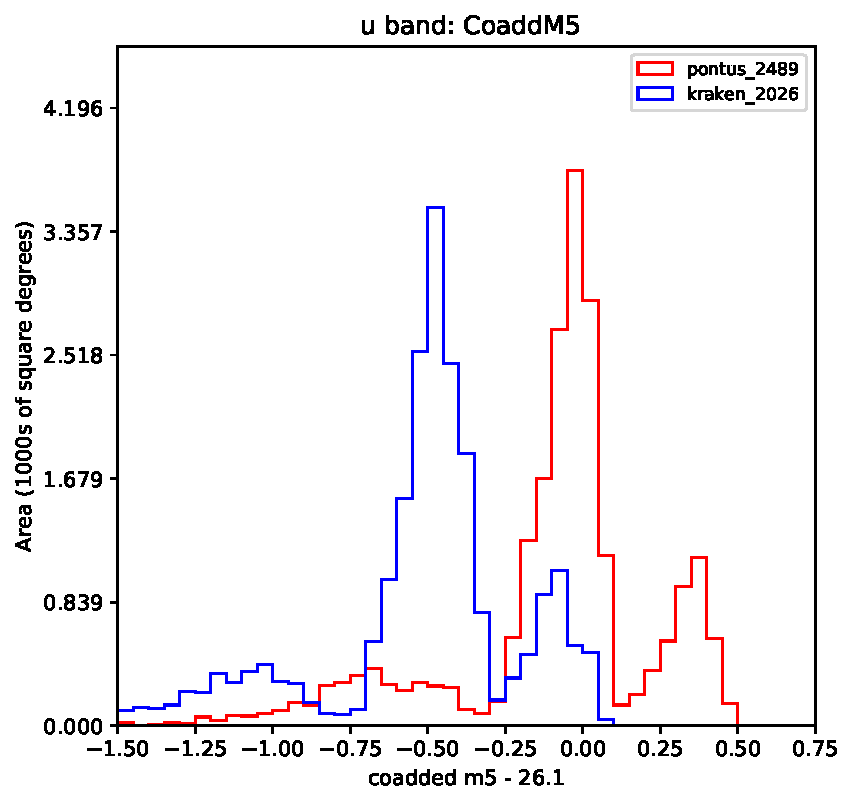
\includegraphics[width=0.65\textwidth]{figures/pontus_2489_kraken_2026_CoaddM5_u_band_HEAL_ComboHistogram.pdf}
%\vskip -1.3in
\caption{Coadded u band magnitude HealPix histograms.}
\label{fig:ubandhist-2489}
\end{figure}

\begin{figure}[ht]
\centering
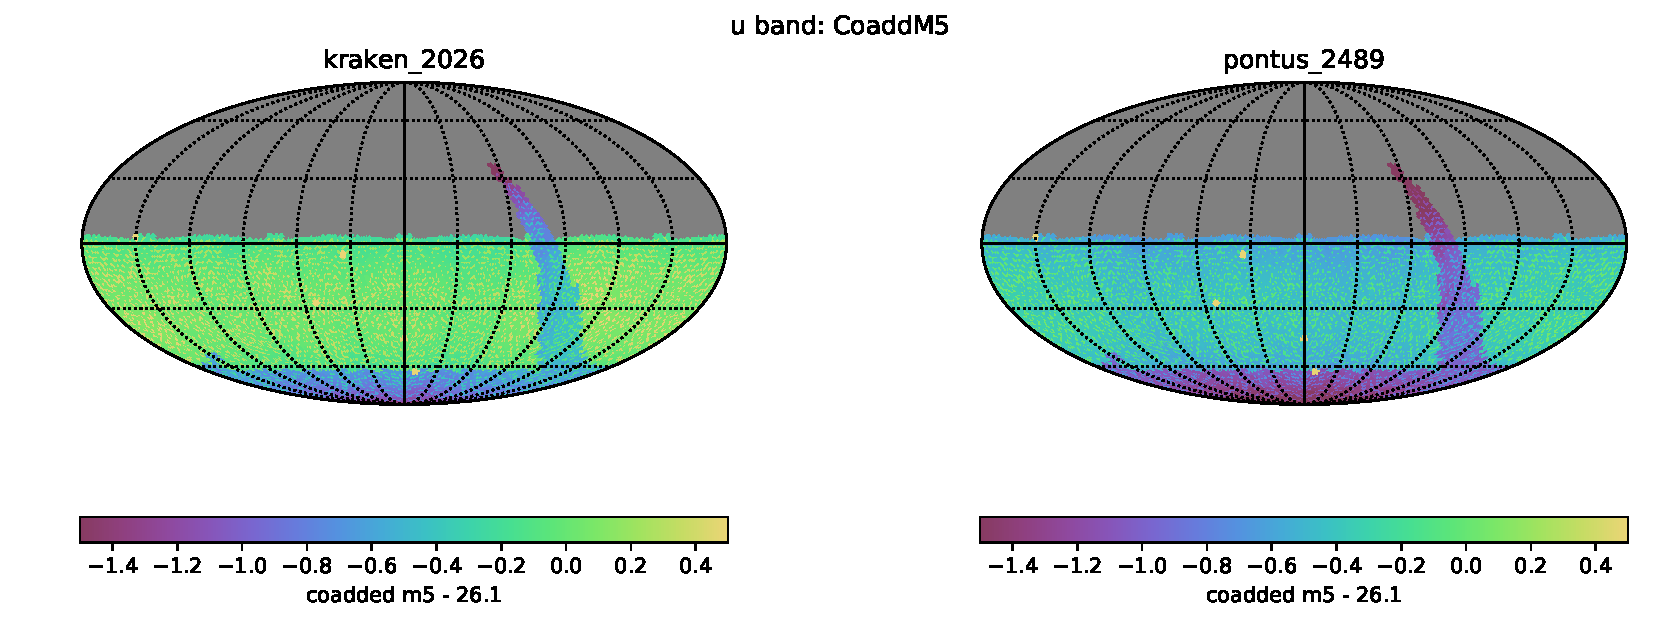
\includegraphics[width=0.98\textwidth]{figures/pontus_2489_kraken_2026_CoaddM5_u_band_HEAL_ComboSkyMap.pdf} 
%\vskip -1.3in
\caption{Coadded u band magnitude HealPix sky maps.}
\label{fig:ubandmap-2489}
\end{figure}

  
\textbf{Conclusions:}  Reducing visits to a single 20 second snap in g,r,i,z,y and 40 second snap in u greatly increased
the number visits and reached a much deeper coadded depth in u. The other aspects of the survey remained relatively
unchanged relative to kraken\_2026.


\subsection{kraken\_2035}  \label{kraken2035}

\textbf{Baseline cadence with 9 Deep Drilling Fields.}

\textbf{Motivation and description:} This survey was used to test the effect of adding 5 additional 
DDFs to the 4 that have been already chosen. The observing cadence in these 5 additional DDFs
was not changed from what was previously used. New fields were not selected with a
particular science goal in mind, but an attempt was made to evenly distribute them in Ra, avoid
the Galactic center, and be out of the Galactic plane. The WFD is expected to take $85-95\%$ of
the observing time during the 10 year survey, with the reaming $5-15\%$ being used for the
other mini-surveys: NES, GP, SCP, and DDFs. By analyzing this simulation, we will be able to see
how the increased number of DDFs affects the proposal balance, and the overall survey efficiency. 
In In Table~\ref{tab:ddfs} we list the 9 DDFs used in kraken\_2035. They can also be seen on the
HealPix Sky map of the coadded r band depth shown in Figure \autoref{fig:rbandmap-2035}.

\begin{table}[htp]
\caption{List of DDFs used in kraken\_2035. The Field IDs with an * are the four already decided fields.}
\begin{center}
\small
\begin{tabular}{lrrrr}
\toprule
Field ID & Ra (Deg) & Dec (Deg) & Galactic l & Galactic b \\
\midrule
290  & 349.386443 & -63.321004 & 319.34 & -50.71 \\
$744^{*}$  &   0.0      & -45.524505 & 328.66 & -68.95 \\
820  & 119.555145 & -43.366522 & 258.34 & -7.31 \\
858  & 187.624779 & -42.492805 & 298.82 &  20.21 \\
1200 & 176.62637  & -33.146604 & 287.59 &  27.78 \\
$1427^{*}$ & 53.009145  & -27.438943 & 222.92 & -54.48 \\
$2412^{*}$ & 34.393398  & -5.09032   & 169.72 & -59.89 \\
2689 & 201.854221 &  0.931384  & 322.66 &  62.42 \\
$2786^{*}$ & 150.362355 &  2.836499  & 236.32 &  42.68 \\
\bottomrule
\end{tabular}
\end{center}
\label{tab:ddfs}
\end{table}

\begin{figure}[ht]
\centering
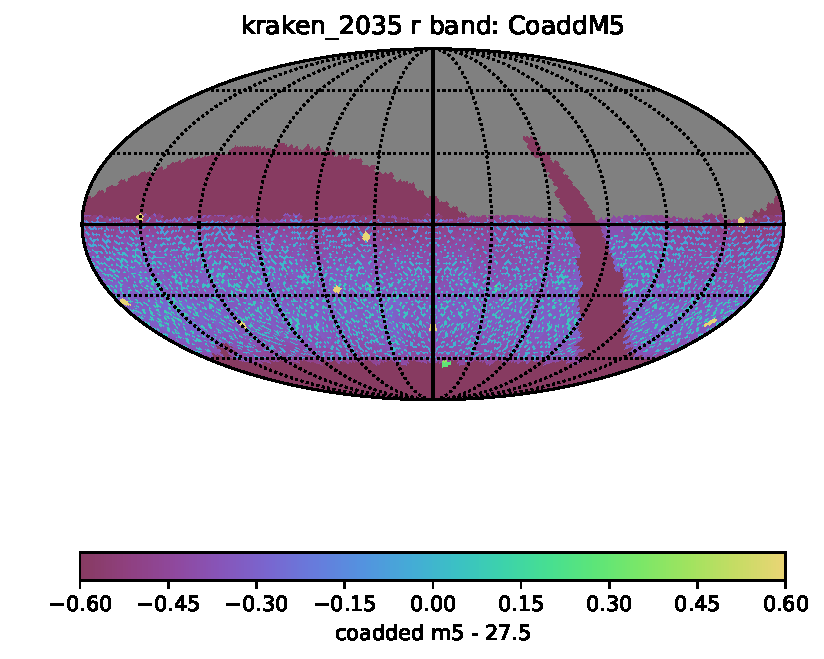
\includegraphics[width=0.65\textwidth]{figures/kraken_2035_CoaddM5_r_band_HEAL_SkyMap.pdf} 
%\vskip -1.3in
\caption{Coadded r band magnitude HealPix sky maps.}
\label{fig:rbandmap-2035}
\end{figure}

\textbf{Analysis and Results: Comparison of kraken\_2035 to kraken\_2026:}

\begin{enumerate}
\item The total number of visits in kraken\_2035 is decreased by 1.2$\%$ relative to kraken\_2026.
\item The WFD only makes up 84$\%$ of the total number of visits, compared to 86$\%$ in kraken\_2026.
\item The DDFs makes up 7$\%$ of the total number of visits, compared to 5$\%$ in kraken\_2026.
\item The rest of the proposal contributions remain approximately the same.
\item The median number of visits in all bands in the WFD decreases by 3$\%$.
\item kraken\_2035 still passed the fO SRD metrics.
\item The mean slew time kraken\_2035 is longer than kraken\_2026 (7.3 vs 6.8 sec). 
See Figure \autoref{fig:slew-2035} for the slew time histograms of each run.
\item The total number of filter changes during the whole survey increases by 30$\%$ relative to kraken\_2026.
\item The median coadded $5\sigma$ depths for the DDFs are (27.7, 28.7, 28.7, 28.2, 27.8, 26.6) in the $ugrizy$ bands, respectively.
These values are similar to what was seen in kraken\_2026. The coadded HealPix sky maps for all bands in the DDFs are shown in
 Figure \autoref{fig:ddcoad-2035}.
\item The other major aspects of the survey remain relatively unchanged.

\end{enumerate}


\begin{figure}[ht]
\centering
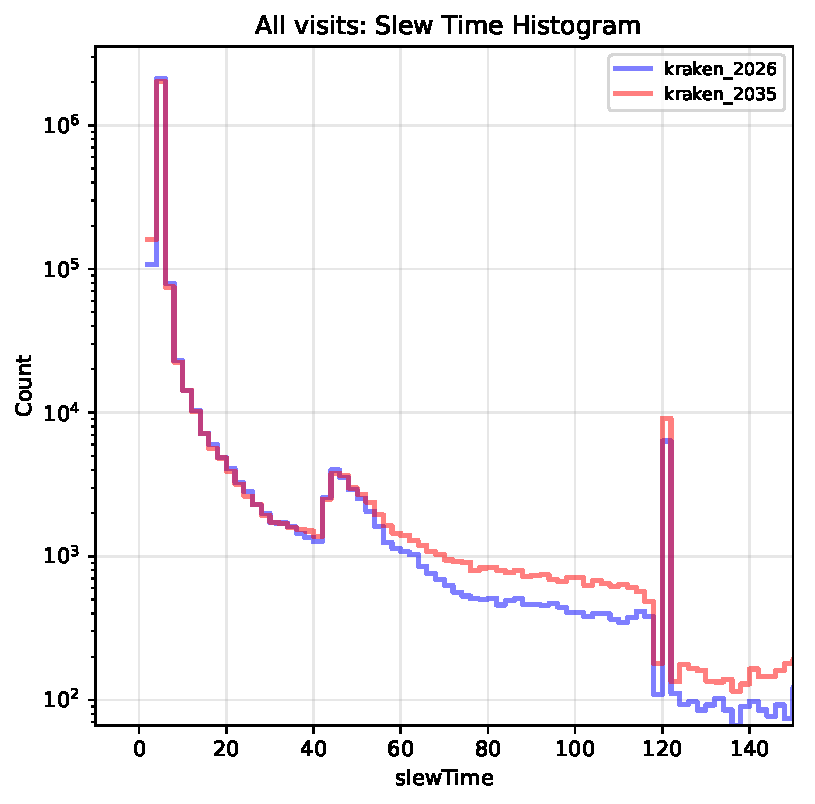
\includegraphics[width=0.65\textwidth]{figures/kraken_2035_kraken_2026_Slew_Time_Histogram_All_visits_ONED_ComboBinnedData.pdf}
%\vskip -1.3in
\caption{Slew time histograms for kraken\_2035 and kraken\_2026 .}
\label{fig:slew-2035}
\end{figure}

\textbf{Conclusions:} Increasing the number of DDFs shifted the proposal distributions with approximately 2$\%$ of WFD visits going
to the DDFs. This shift in visits into the DDFs reduced the WFD fraction just below the nominal limit of $85\%$. The mean slew time
was likely increased in part by the 30$\%$  increase in total filter changes, which in turn reduced the total number of visits. More detailed
metrics aimed at DDFs still need to be developed to understand their performance, and how increasing the total number of fields might
hurt, or improve, the science goals of the DDFs.

\begin{figure}[ht]
\centering
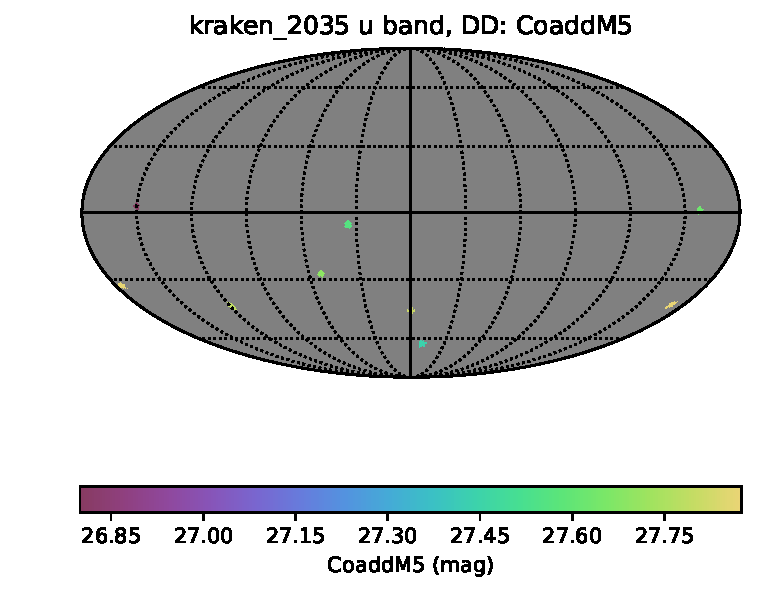
\includegraphics[width=0.43\textwidth]{figures/kraken_2035_CoaddM5_u_band_DD_HEAL_SkyMap.pdf}
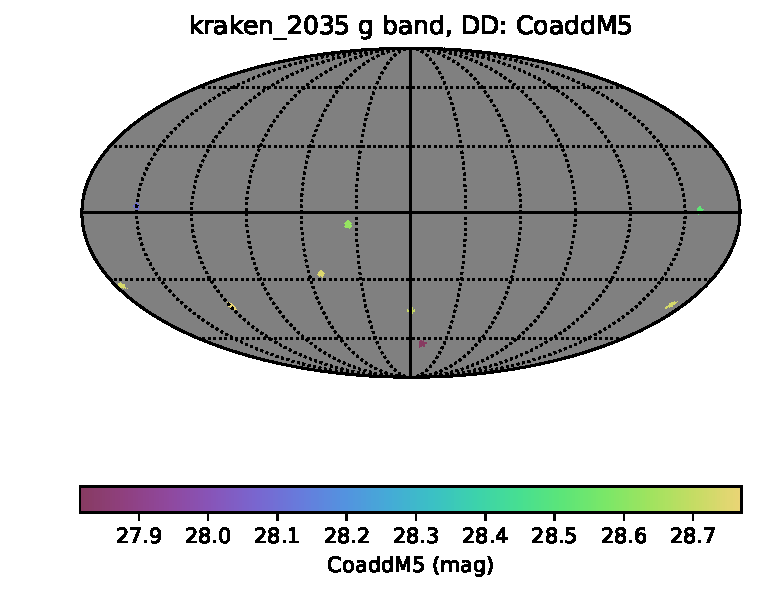
\includegraphics[width=0.43\textwidth]{figures/kraken_2035_CoaddM5_g_band_DD_HEAL_SkyMap.pdf} \\
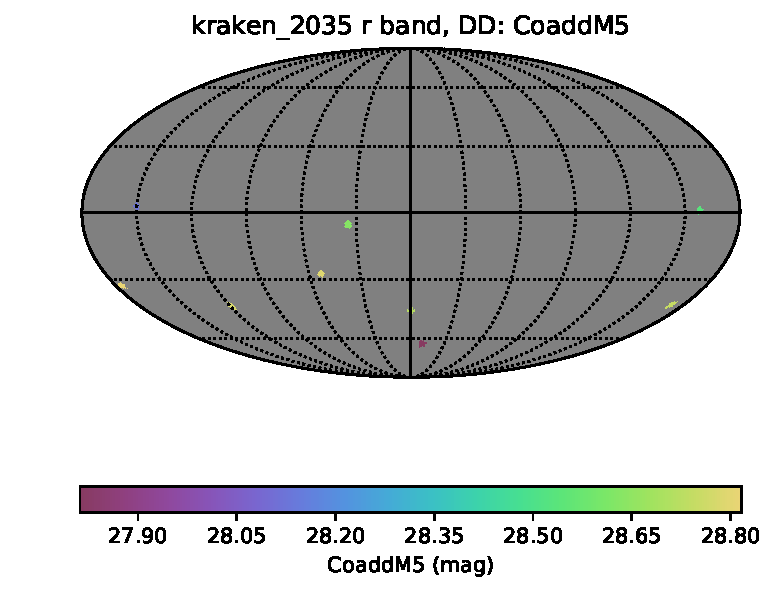
\includegraphics[width=0.43\textwidth]{figures/kraken_2035_CoaddM5_r_band_DD_HEAL_SkyMap.pdf}
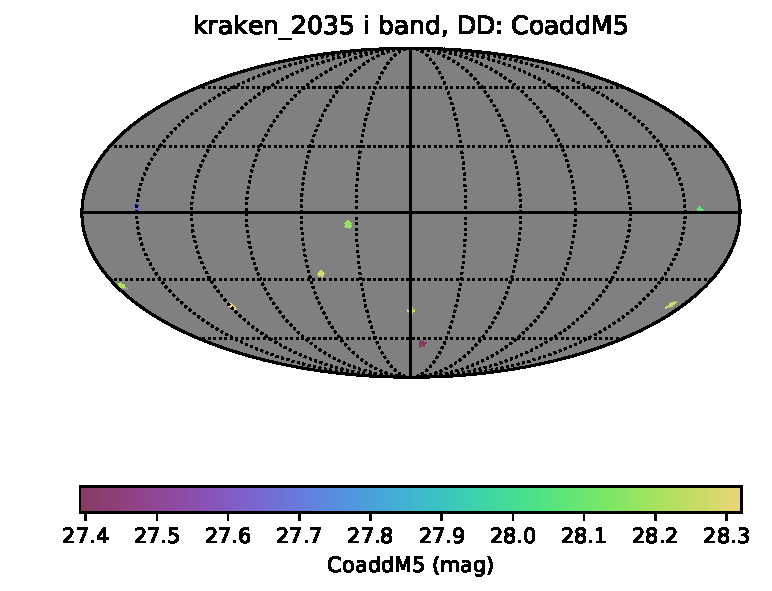
\includegraphics[width=0.43\textwidth]{figures/kraken_2035_CoaddM5_i_band_DD_HEAL_SkyMap.pdf} \\
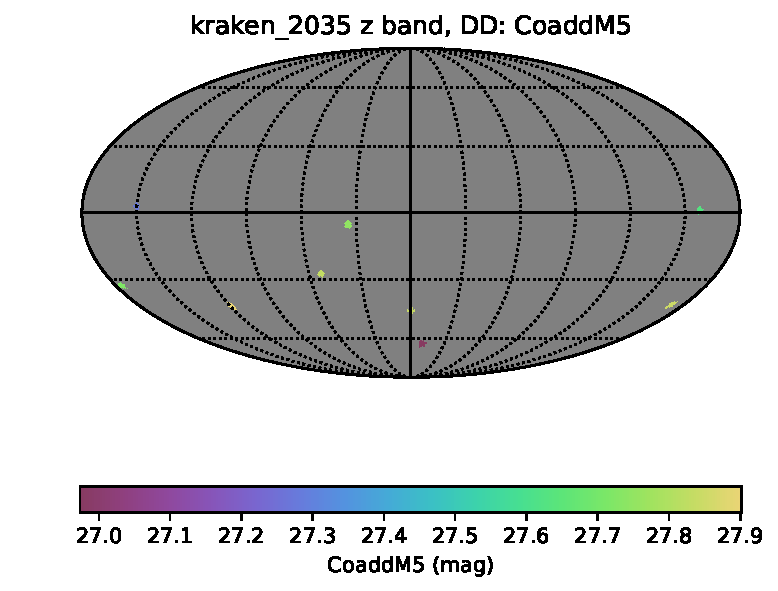
\includegraphics[width=0.43\textwidth]{figures/kraken_2035_CoaddM5_z_band_DD_HEAL_SkyMap.pdf}
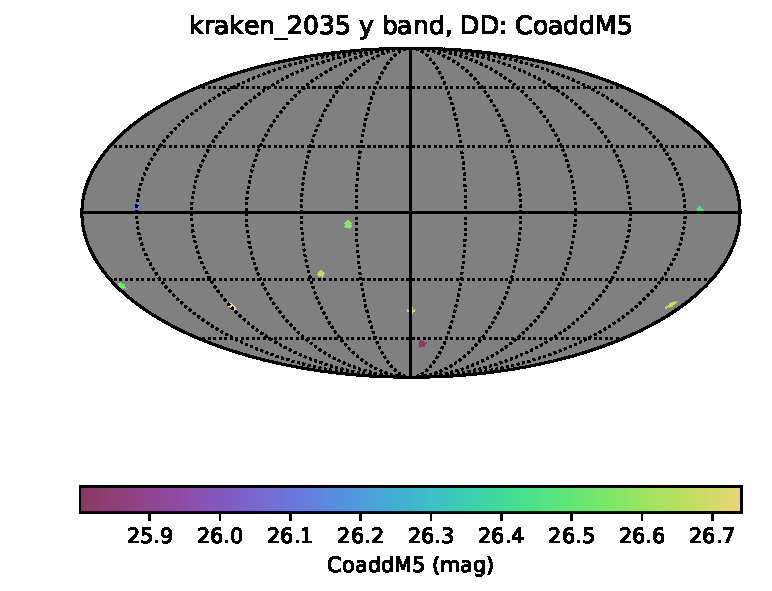
\includegraphics[width=0.43\textwidth]{figures/kraken_2035_CoaddM5_y_band_DD_HEAL_SkyMap.pdf}
\caption{Coadded depths in all bands for DDFs in kraken\_2035 .}
\label{fig:ddcoad-2035}
\end{figure}

\clearpage

\section{Rolling cadence simulations}

\subsection{Overview}

Here we present three simulations that were run with different flavors of a rolling cadence in the WFD survey area.
The idea of implementing a rolling cadence is to increase the temporal sampling of fields in the WFD by turning
regions of the available sky on/off over the course of a survey. When a single area of the sky is turned on for 
enhanced sampling, it is called a ``roll''. In the rolling cadences presented here, we constructed relatively simple
rolls defined by bands in declination that alternate each year of the survey. We also explore the
effect of leaving some fraction of the non-rolling WFD cadence on in addition to rolling declination bands.
It should be noted that these rolling cadence are still very a much a work in progress and should only
serve as a starting point for constructing better rolling cadence experiments. In the future we will also develop more
complicated rolls that depend on more than just declination. We are also still in the process of developing new
metrics for MAF that test the efficiency and benefit of the rolling cadences. It is difficult to make a direct comparison
of the rolling cadences to kraken\_2026, but we will provide some overall insights in this section. There are many
more issues with each of these surveys that can be seen in there total MAF output (URL), but going into
all of the details there is beyond the scope of this document.

\subsection{mothra\_2045} \label{mothra2045}

\textbf{Two rolling dec bands, no non-rolling WFD included}

\textbf{Motivation and description:} This simulations represents one of the simplest implementations of a rolling cadence:
two dec bands (northern and southern) that alternate every year for the entire survey. In mothra\_2045, the southern dec band extended from 
from $-62.5^{\circ}$ to $-24.7^{\circ}$, and the northern dec extends from $-24.7^{\circ}$ to $2.8^{\circ}$. The simulation started with
the southern dec band for year 1 and then alternated every year until the end of the survey. In Figure \autoref{fig:rolling_nvis-2045}
we plot the number of visits over the first four years of the survey to illustrate the locations of the rolls and when they are active.

\textbf{Analysis and Results: Comparison of mothra\_2045 to kraken\_2026:}

\begin{enumerate}
\item The total number of visits in mothra\_2045 decreases by 26$\%$ relative to kraken\_2026.
\item The WFD only makes up 83$\%$ of the total number of visits, compared to 86$\%$ in kraken\_2026.
The SCP and NES increased their fraction of the total survey by approximately 2$\%$.
\item The mean slew time kraken\_2035 is longer than kraken\_2026 (16.19 vs 6.8 sec). 
\item The total number of filter changes during the whole survey increases by 144$\%$ relative to kraken\_2026.
\item The median number of visits per night mothra\_2045 lower than kraken\_2026 (618 vs 806). 
\item The median inter-night gap for all WFD visits in mothra\_2045 is shorter than in kraken\_2026 by nearly one night (1.01 vs 1.96).
\end{enumerate}

\begin{figure}[ht]
\centering
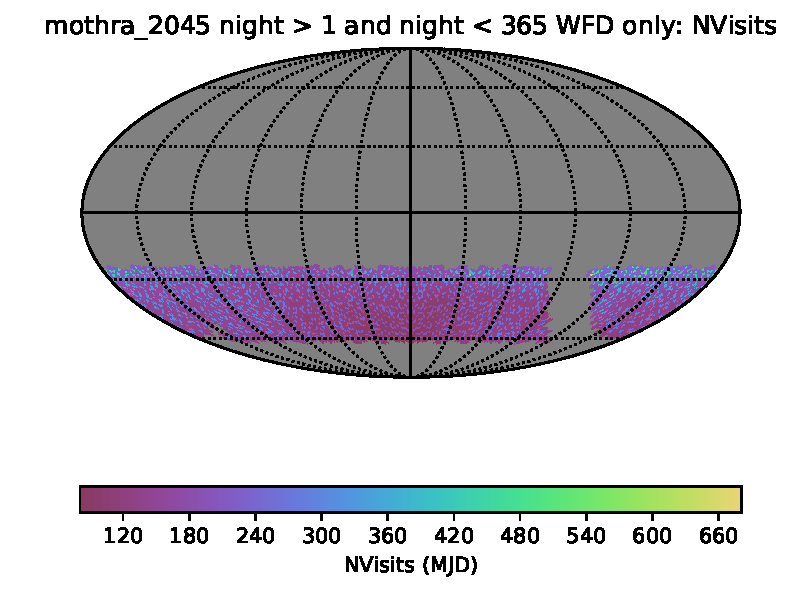
\includegraphics[width=0.45\textwidth]{figures/mothra_2045_NVisits_night_gt_1_and_night_lt_365_WFD_only_HEAL_SkyMap.pdf}
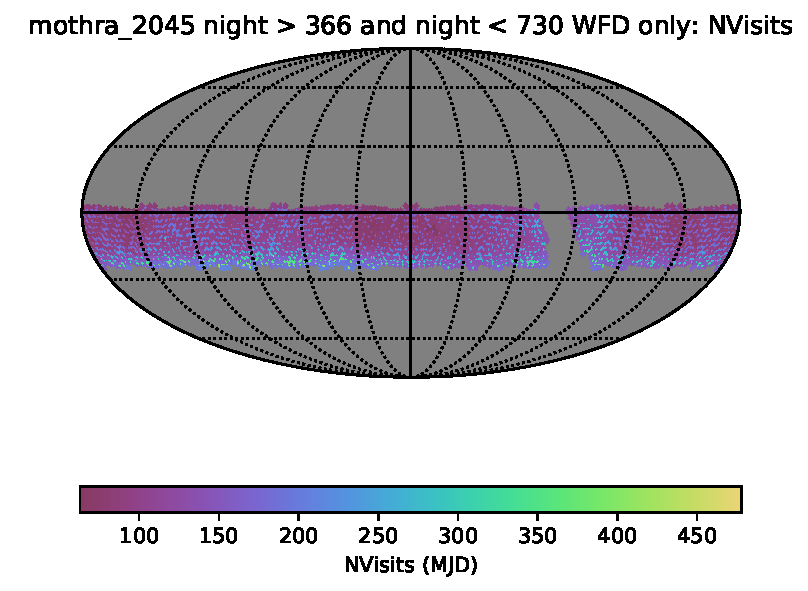
\includegraphics[width=0.45\textwidth]{figures/mothra_2045_NVisits_night_gt_366_and_night_lt_730_WFD_only_HEAL_SkyMap.pdf}\\
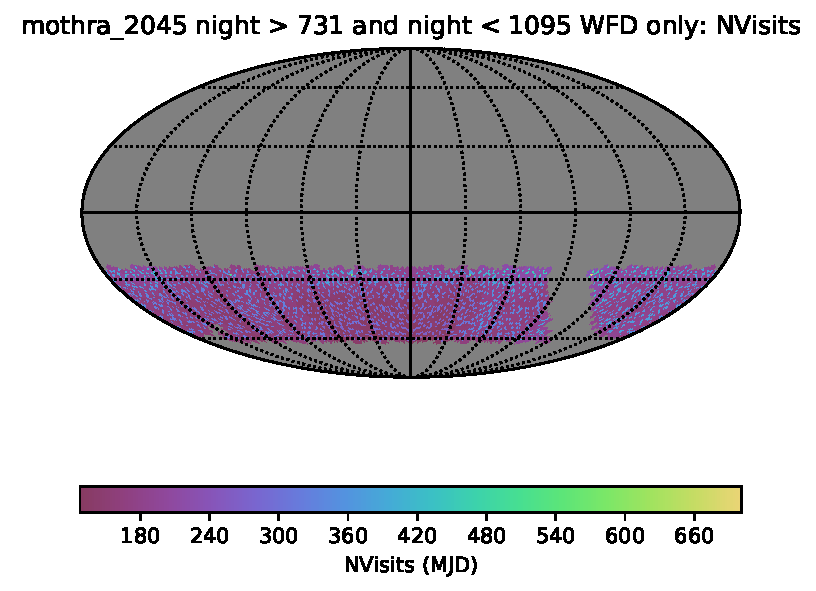
\includegraphics[width=0.45\textwidth]{figures/mothra_2045_NVisits_night_gt_731_and_night_lt_1095_WFD_only_HEAL_SkyMap.pdf}
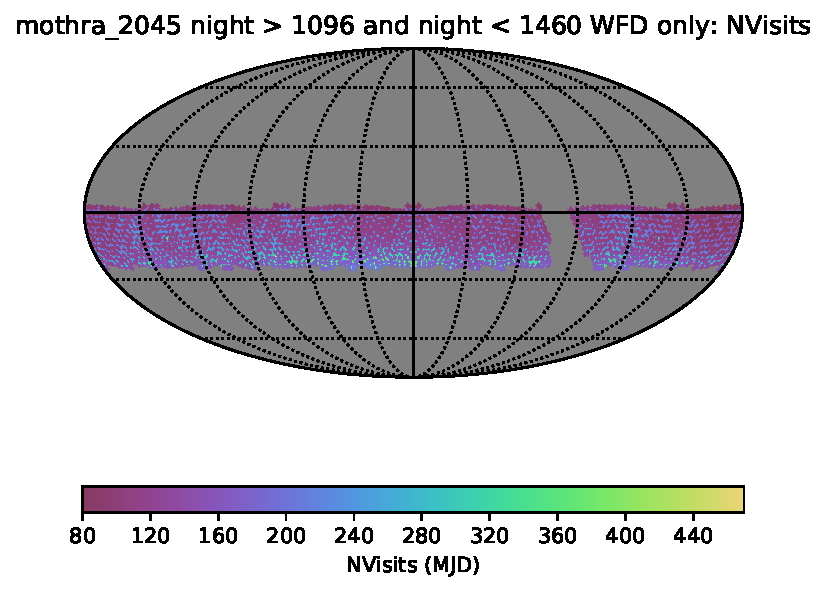
\includegraphics[width=0.45\textwidth]{figures/mothra_2045_NVisits_night_gt_1096_and_night_lt_1460_WFD_only_HEAL_SkyMap.pdf}
\caption{First 4 years of rolling WFD observations in  mothra\_2045.}
\label{fig:rolling_nvis-2045}
\end{figure}

\textbf{Conclusions:} There are obviously many issues with mothra\_2045 that leave room for improvement. The shorter median inter-night
gap compared to kraken\_2026 shows that the rolling cadence is increasing the temporal sampling in the WFD, but we still need to determine
the best way to balance that with the other surveys.

\subsection{pontus\_2502} \label{pontus2502}

\textbf{Motivation and description:} This simulations uses the same two rolling dec bands from mothra\_2045, but also has the
regular WFD cadence at a $25\%$ level on at all times. To make this configuration, $75\%$ of the total visits needed in the WFD area are requested from the
rolling dec bands, and the remaining $25\%$ from the non-rolling WFD cadence. The configuration was done so that the rolling and non-rolling WFD 
proposals could not co-add their weights when selecting the next target in the simulation. In Figure \autoref{fig:rolling_nvis-2502} we plot the number 
of visits over the first four years of the survey to illustrate the locations of the rolls and when they are active. By comparing \autoref{fig:rolling_nvis-2502} 
to \autoref{fig:rolling_nvis-2045} you can get a sense for how pontus\_2502 differs from mothra\_2045.

\textbf{Analysis and Results: Comparison of pontus\_2502 to kraken\_2026:}


\begin{enumerate}
\item The total number of visits in pontus\_2502 decreases by 17$\%$ relative to kraken\_2026.
\item The total WFD area makes up 89$\%$ of the total number of visits, compared to 86$\%$ in kraken\_2026.
59$\%$ percent of the visits were from the rolling dec bands, and 31$\%$ were from the non-rolling WFD proposal.
\item The DDFs only made up  0.3$\%$ of all visits suggesting that the proposals need better balancing. 
\item The mean slew time in pontus\_2502 is longer than kraken\_2026 (7.86 vs 6.8 sec). 
\item The total number of filter changes during the whole survey increased by 18$\%$ relative to kraken\_2026.
\item The median number of visits per night in pontus\_2502 is lower than kraken\_2026 (721 vs 806). 
\item The median inter-night gap for all WFD visits in pontus\_2502 is basically the same as kraken\_2026  (1.88 vs 1.96).
\end{enumerate}

\begin{figure}[ht]
\centering
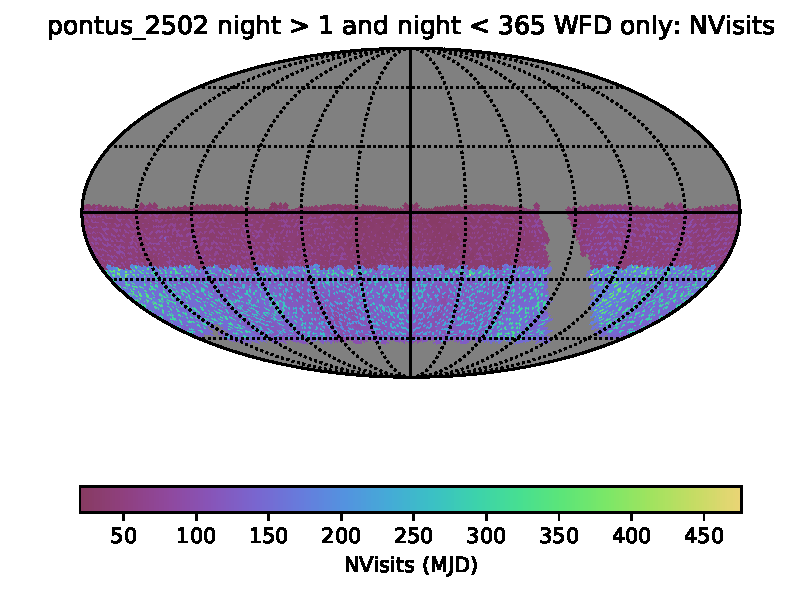
\includegraphics[width=0.45\textwidth]{figures/pontus_2502_NVisits_night_gt_1_and_night_lt_365_WFD_only_HEAL_SkyMap.pdf}
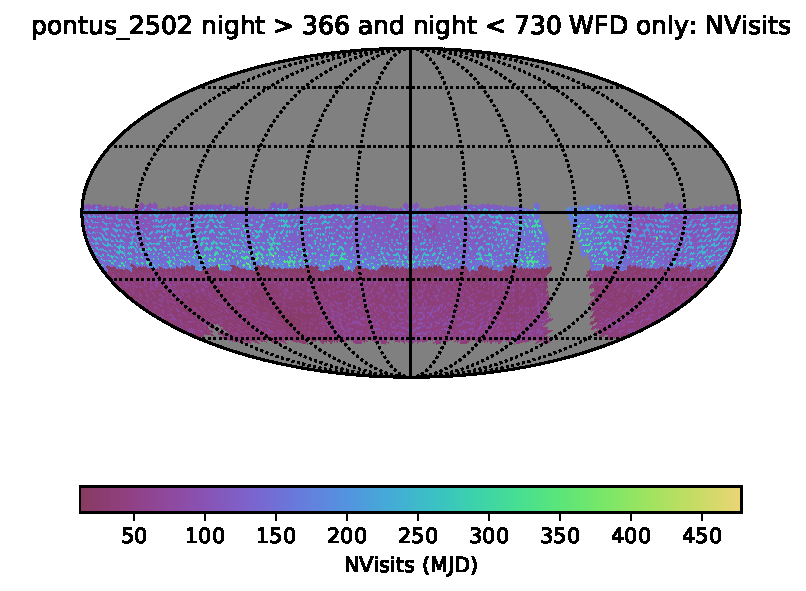
\includegraphics[width=0.45\textwidth]{figures/pontus_2502_NVisits_night_gt_366_and_night_lt_730_WFD_only_HEAL_SkyMap.pdf}\\
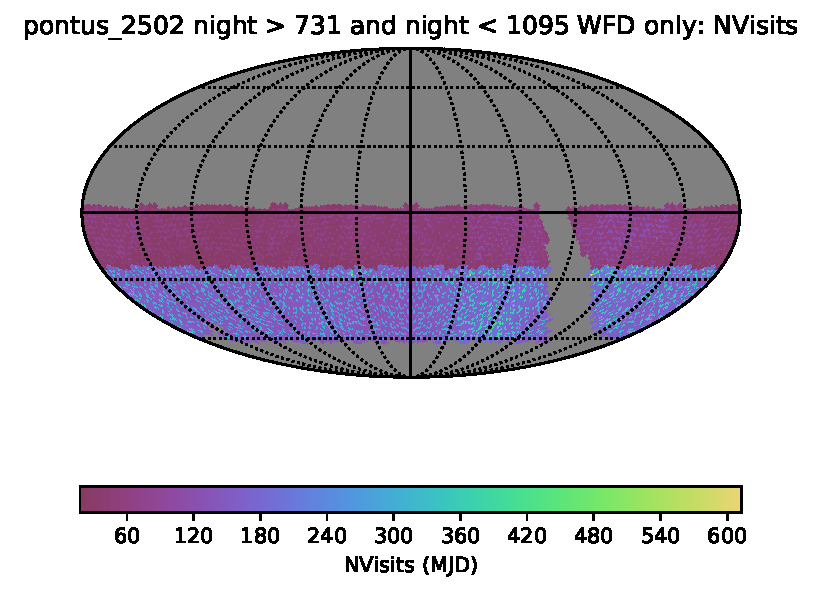
\includegraphics[width=0.45\textwidth]{figures/pontus_2502_NVisits_night_gt_731_and_night_lt_1095_WFD_only_HEAL_SkyMap.pdf}
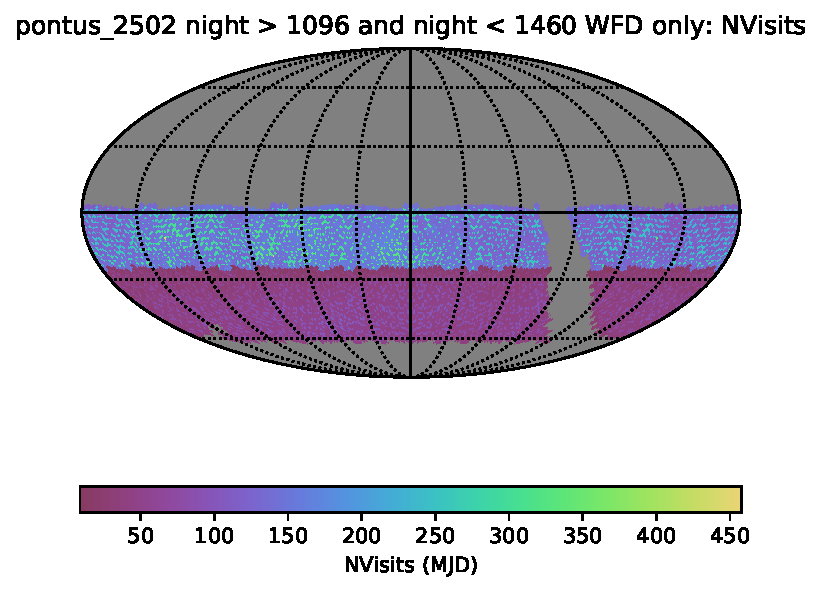
\includegraphics[width=0.45\textwidth]{figures/pontus_2502_NVisits_night_gt_1096_and_night_lt_1460_WFD_only_HEAL_SkyMap.pdf}
\caption{First 4 years of rolling WFD observations in  pontus\_2502.}
\label{fig:rolling_nvis-2502}
\end{figure}

\textbf{Conclusions:} Including the non-rolling WFD cadence at $25\%$ improved some aspects of the survey 
relative to mothra\_2045, which had the non-rolling WFD completely turned off. We saw an increase in the number of visits,
and decreases in the number of filter changes and mean slew times. This run did have the major issue that the DDFs only
make up a fraction of a percent of the total number visits. There was also not a large improvement in the median-inter night
gap relative to kraken\_2026, which is one of the main goals of using a rolling cadence.

\subsection{kraken\_2036} \label{kraken2036}

\textbf{Three rolling dec bands}

\textbf{Motivation and description:} In this simulation we take a different approach approach to the rolling cadence. During
the first and last to years of the survey, the full area of the WFD is available for observations ($-62.5^{\circ}$ to $2.8^{\circ}$), so essentially
operating at the usual WFD cadence. For the remaining six years, the WFD region is broken up into three dec bands that alternate every year,
so each of the three dec bands is turned on twice during the 10 year survey. In Figure \autoref{fig:rolling_nvis-2036}
we plot the number of visits over the first five years of the survey to illustrate the locations of the rolls and when they are active. Note that
the upper left panel in Figure \autoref{fig:rolling_nvis-2036} covers two years of the sruvey.

\begin{figure}[ht]
\centering
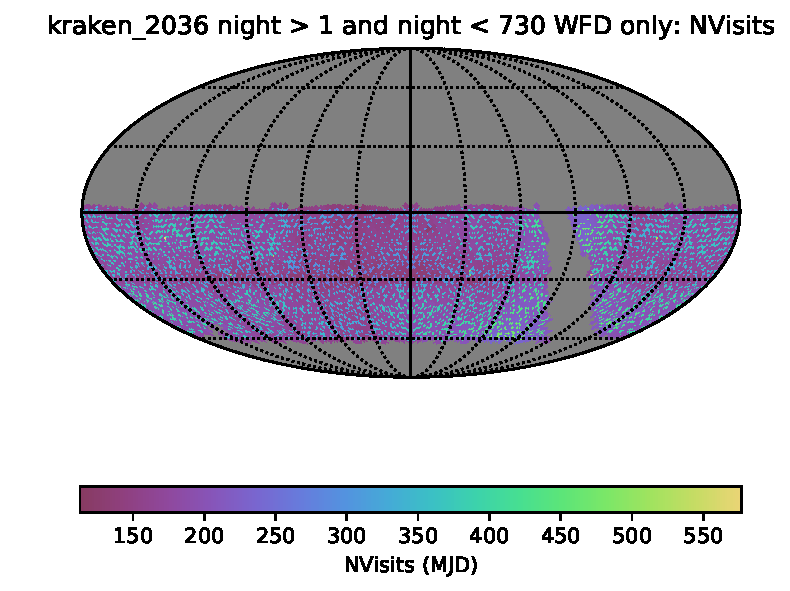
\includegraphics[width=0.45\textwidth]{figures/kraken_2036_NVisits_night_gt_1_and_night_lt_730_WFD_only_HEAL_SkyMap.pdf}
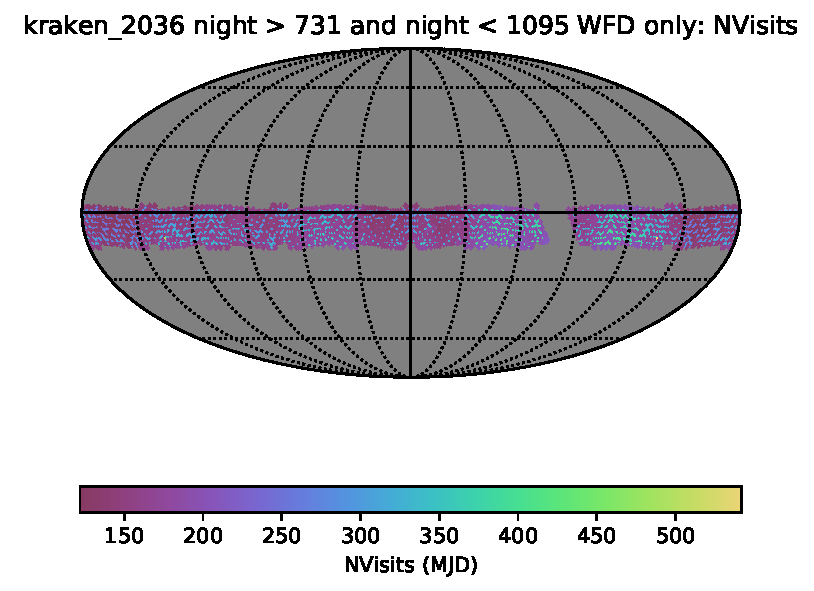
\includegraphics[width=0.45\textwidth]{figures/kraken_2036_NVisits_night_gt_731_and_night_lt_1095_WFD_only_HEAL_SkyMap.pdf} \\
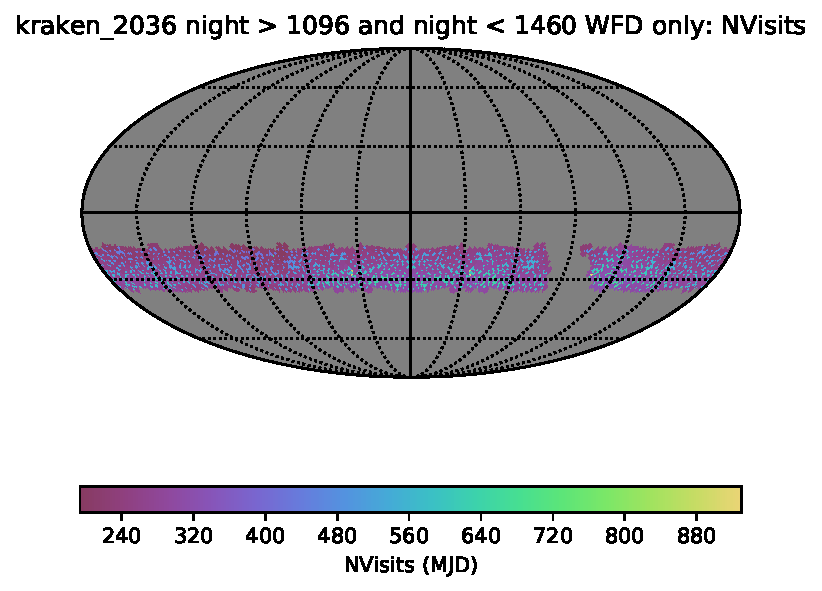
\includegraphics[width=0.45\textwidth]{figures/kraken_2036_NVisits_night_gt_1096_and_night_lt_1460_WFD_only_HEAL_SkyMap.pdf}
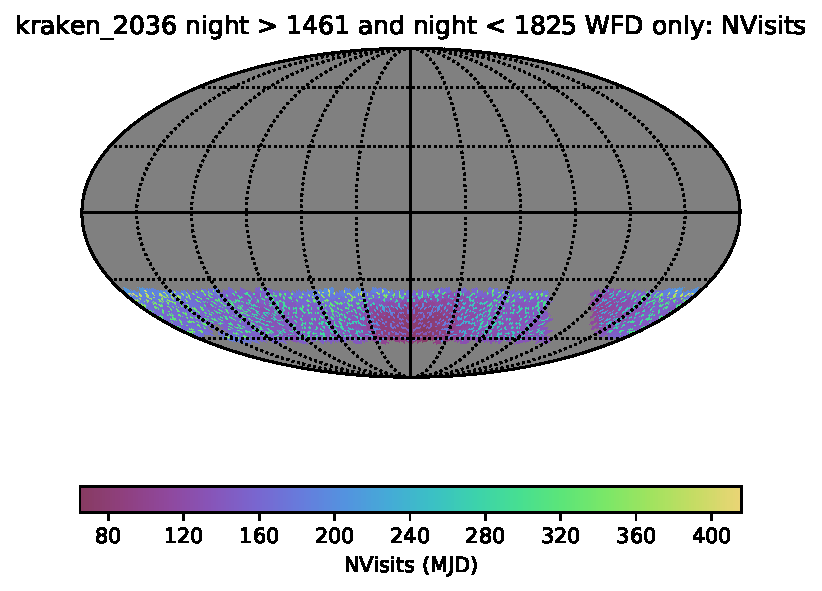
\includegraphics[width=0.45\textwidth]{figures/kraken_2036_NVisits_night_gt_1461_and_night_lt_1825_WFD_only_HEAL_SkyMap.pdf}
\caption{First 5 years of rolling WFD observations in  kraken\_2036.}
\label{fig:rolling_nvis-2036}
\end{figure}

\textbf{Analysis and Results: Comparison of kraken\_2036 to kraken\_2026:}

\begin{enumerate}
\item The total number of visits in kraken\_203 decreases by 15$\%$ relative to kraken\_2026. This is the best performance
of the rolling cadences presented here.
\item The total WFD area makes up 85$\%$ of the total number of visits, compared to 86$\%$ in kraken\_2026.
\item The remaining proposal fractions are similar to what is seen in kraken\_2026.
\item The mean slew time kraken\_2036 is longer than kraken\_2026 (12.61 vs 6.8 sec). The slew time and slew distance
histograms are shown in Figure \autoref{fig:slews-2036}. From these histograms we can see that kraken\_2036 is making longer
slews in distance and time, which is likely due to jumping between the dec bands and area proposals.
\item The total number of filter changes during the whole survey increases by 70$\%$ relative to kraken\_2026.
\item The median number of visits per night kraken\_2036 lower than kraken\_2026 (721 vs 806). 
\item The median inter-night gap for all WFD visits in kraken\_2036 is shorter than in kraken\_2026 by nearly one night (1.01 vs 1.96).
\end{enumerate}


\begin{figure}[ht]
\centering
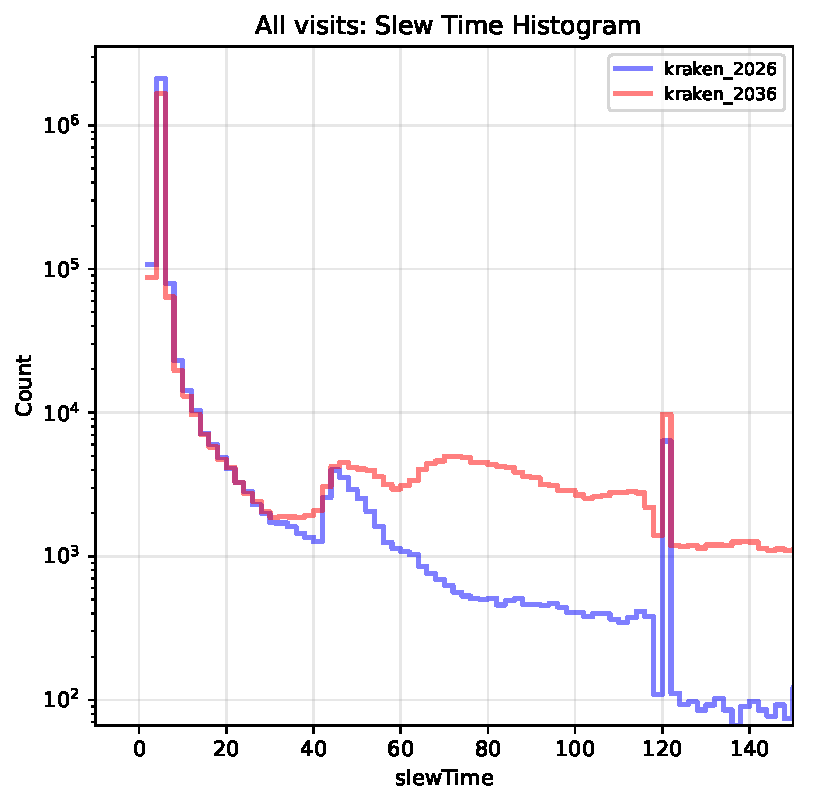
\includegraphics[width=0.45\textwidth]{figures/kraken_2026_kraken_2036_Slew_Time_Histogram_All_visits_ONED_ComboBinnedData.pdf}
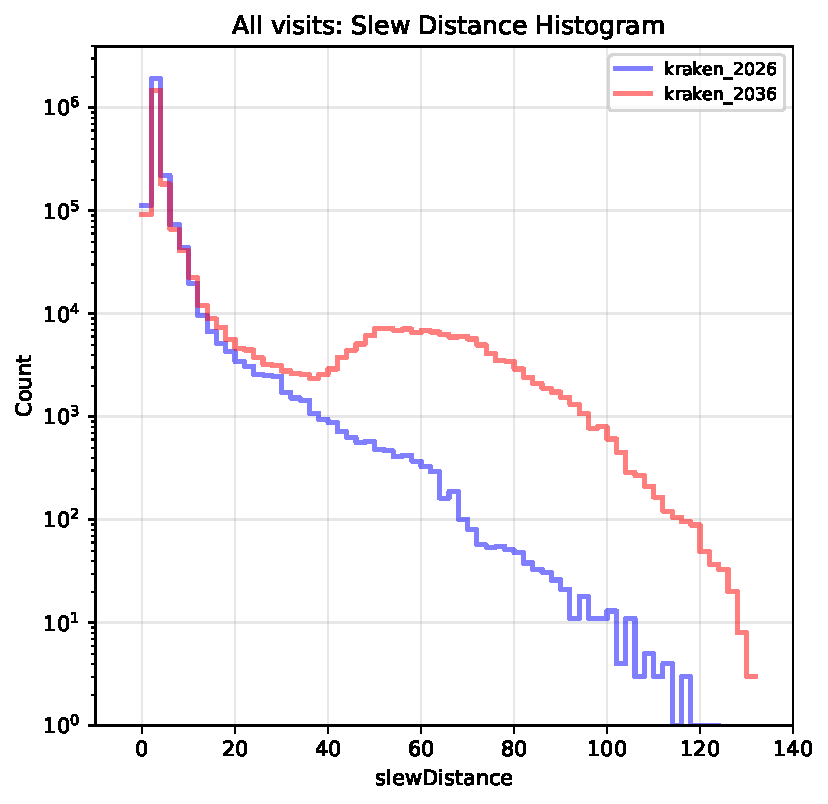
\includegraphics[width=0.45\textwidth]{figures/kraken_2026_kraken_2036_Slew_Distance_Histogram_All_visits_ONED_ComboBinnedData.pdf} 
\caption{Slew time and distance histograms for kraken\_2036 and  kraken\_2026.}
\label{fig:slews-2036}
\end{figure}


\textbf{Conclusions:} This simulation performed the best out of the three rolling cadence experiments shown here. We saw the
largest number of visits without drastically changing the distribution of visits among the various proposals, and a 
significant decrease in the median inter-night gap relative to the non-rolling baseline. Like the other rolling cadences, however, 
there is still room a lot for improvement in how cadences such as this are implemented. 


% Include all the relevant bib files.
% https://lsst-texmf.lsst.io/lsstdoc.html#bibliographies
% Set up the LSST texmf package to get these bibtex files.
%\bibliography{lsst,lsst-dm,refs_ads,refs,books}

\end{document}
